% %%%%%%%%%%%%%%%%%%%%%%%%%%%%%%%%%%%%%%%%%%%%%%%%%%%%%%%%%%%%%%%%%%%%%%%%%%%%%%%%%%%%%%%%%%%%
% PROBLEM SET LATEX TEMPLATE FILE
% DEFINE DOCUMENT STYLE, LOAD PACKAGES
\documentclass[11pt,notitlepage]{article}\usepackage[]{graphicx}\usepackage[]{color}
%% maxwidth is the original width if it is less than linewidth
%% otherwise use linewidth (to make sure the graphics do not exceed the margin)
\makeatletter
\def\maxwidth{ %
  \ifdim\Gin@nat@width>\linewidth
    \linewidth
  \else
    \Gin@nat@width
  \fi
}
\makeatother

\definecolor{fgcolor}{rgb}{0.345, 0.345, 0.345}
\newcommand{\hlnum}[1]{\textcolor[rgb]{0.686,0.059,0.569}{#1}}%
\newcommand{\hlstr}[1]{\textcolor[rgb]{0.192,0.494,0.8}{#1}}%
\newcommand{\hlcom}[1]{\textcolor[rgb]{0.678,0.584,0.686}{\textit{#1}}}%
\newcommand{\hlopt}[1]{\textcolor[rgb]{0,0,0}{#1}}%
\newcommand{\hlstd}[1]{\textcolor[rgb]{0.345,0.345,0.345}{#1}}%
\newcommand{\hlkwa}[1]{\textcolor[rgb]{0.161,0.373,0.58}{\textbf{#1}}}%
\newcommand{\hlkwb}[1]{\textcolor[rgb]{0.69,0.353,0.396}{#1}}%
\newcommand{\hlkwc}[1]{\textcolor[rgb]{0.333,0.667,0.333}{#1}}%
\newcommand{\hlkwd}[1]{\textcolor[rgb]{0.737,0.353,0.396}{\textbf{#1}}}%

\usepackage{framed}
\makeatletter
\newenvironment{kframe}{%
 \def\at@end@of@kframe{}%
 \ifinner\ifhmode%
  \def\at@end@of@kframe{\end{minipage}}%
  \begin{minipage}{\columnwidth}%
 \fi\fi%
 \def\FrameCommand##1{\hskip\@totalleftmargin \hskip-\fboxsep
 \colorbox{shadecolor}{##1}\hskip-\fboxsep
     % There is no \\@totalrightmargin, so:
     \hskip-\linewidth \hskip-\@totalleftmargin \hskip\columnwidth}%
 \MakeFramed {\advance\hsize-\width
   \@totalleftmargin\z@ \linewidth\hsize
   \@setminipage}}%
 {\par\unskip\endMakeFramed%
 \at@end@of@kframe}
\makeatother

\definecolor{shadecolor}{rgb}{.97, .97, .97}
\definecolor{messagecolor}{rgb}{0, 0, 0}
\definecolor{warningcolor}{rgb}{1, 0, 1}
\definecolor{errorcolor}{rgb}{1, 0, 0}
\newenvironment{knitrout}{}{} % an empty environment to be redefined in TeX

\usepackage{alltt}    % ADD COMMENTS USING A PERCENT SIGN
\usepackage{amsfonts}
\usepackage{amsthm}
\usepackage{amsmath, booktabs}
\usepackage{mathtools}
\usepackage{amssymb}
\usepackage{subfig}
\usepackage{setspace}
\usepackage{fullpage}
\usepackage{verbatim}
\usepackage{graphicx}
\usepackage{tabularx}
\usepackage{longtable}
\usepackage{multicol}
\usepackage{multirow}
\setlength{\parindent}{0in}  	% uncomment to remove indent at start of paragraphs
\usepackage{pdflscape}
\usepackage[english]{babel}
\usepackage[pdftex]{hyperref}
\usepackage{natbib}
\usepackage{caption}
\usepackage{amsmath}
\usepackage{amsfonts}
\usepackage{graphics}
\usepackage{multirow}
\usepackage{graphics}
\usepackage{hyperref}
\usepackage{longtable}
\usepackage{latexsym}
\usepackage{rotating}
\usepackage{setspace}
\usepackage{layouts} 
\usepackage[titletoc]{appendix}
\DeclareGraphicsExtensions{.pdf,.jpg,.png}
\usepackage[margin=1in]{geometry}
\usepackage{enumerate}
\usepackage{float}

\newcolumntype{L}[1]{>{\raggedright\let\newline\\\arraybackslash\hspace{0pt}}m{#1}}
\newcolumntype{C}[1]{>{\centering\let\newline\\\arraybackslash\hspace{0pt}}m{#1}}
\newcolumntype{R}[1]{>{\raggedleft\let\newline\\\arraybackslash\hspace{0pt}}m{#1}}

\usepackage[T1]{fontenc}				

\usepackage{xcolor}
\usepackage[printwatermark]{xwatermark}
\newwatermark[allpages,color=black!50,angle=45,scale=1,xpos=0,ypos=0]{DO NOT DISTRIBUTE}
\usepackage{textcomp} % defines textquotesingle
 \AtBeginDocument{%
        \def\PYZsq{\textquotesingle}% Upright quotes in Pygmentized code
    }
 
 \usepackage{fancyvrb} % verbatim replacement that allows latex
    % Hack from http://tex.stackexchange.com/a/47451/13684:
    \AtBeginDocument{%
        \def\PYZsq{\textquotesingle}% Upright quotes in Pygmentized code
    }
    \usepackage{upquote} % Upright quotes for verbatim code
 


    % Pygments definitions
    
\makeatletter
\def\PY@reset{\let\PY@it=\relax \let\PY@bf=\relax%
    \let\PY@ul=\relax \let\PY@tc=\relax%
    \let\PY@bc=\relax \let\PY@ff=\relax}
\def\PY@tok#1{\csname PY@tok@#1\endcsname}
\def\PY@toks#1+{\ifx\relax#1\empty\else%
    \PY@tok{#1}\expandafter\PY@toks\fi}
\def\PY@do#1{\PY@bc{\PY@tc{\PY@ul{%
    \PY@it{\PY@bf{\PY@ff{#1}}}}}}}
\def\PY#1#2{\PY@reset\PY@toks#1+\relax+\PY@do{#2}}

\expandafter\def\csname PY@tok@w\endcsname{\def\PY@tc##1{\textcolor[rgb]{0.73,0.73,0.73}{##1}}}
\expandafter\def\csname PY@tok@c\endcsname{\let\PY@it=\textit\def\PY@tc##1{\textcolor[rgb]{0.25,0.50,0.50}{##1}}}
\expandafter\def\csname PY@tok@cp\endcsname{\def\PY@tc##1{\textcolor[rgb]{0.74,0.48,0.00}{##1}}}
\expandafter\def\csname PY@tok@k\endcsname{\let\PY@bf=\textbf\def\PY@tc##1{\textcolor[rgb]{0.00,0.50,0.00}{##1}}}
\expandafter\def\csname PY@tok@kp\endcsname{\def\PY@tc##1{\textcolor[rgb]{0.00,0.50,0.00}{##1}}}
\expandafter\def\csname PY@tok@kt\endcsname{\def\PY@tc##1{\textcolor[rgb]{0.69,0.00,0.25}{##1}}}
\expandafter\def\csname PY@tok@o\endcsname{\def\PY@tc##1{\textcolor[rgb]{0.40,0.40,0.40}{##1}}}
\expandafter\def\csname PY@tok@ow\endcsname{\let\PY@bf=\textbf\def\PY@tc##1{\textcolor[rgb]{0.67,0.13,1.00}{##1}}}
\expandafter\def\csname PY@tok@nb\endcsname{\def\PY@tc##1{\textcolor[rgb]{0.00,0.50,0.00}{##1}}}
\expandafter\def\csname PY@tok@nf\endcsname{\def\PY@tc##1{\textcolor[rgb]{0.00,0.00,1.00}{##1}}}
\expandafter\def\csname PY@tok@nc\endcsname{\let\PY@bf=\textbf\def\PY@tc##1{\textcolor[rgb]{0.00,0.00,1.00}{##1}}}
\expandafter\def\csname PY@tok@nn\endcsname{\let\PY@bf=\textbf\def\PY@tc##1{\textcolor[rgb]{0.00,0.00,1.00}{##1}}}
\expandafter\def\csname PY@tok@ne\endcsname{\let\PY@bf=\textbf\def\PY@tc##1{\textcolor[rgb]{0.82,0.25,0.23}{##1}}}
\expandafter\def\csname PY@tok@nv\endcsname{\def\PY@tc##1{\textcolor[rgb]{0.10,0.09,0.49}{##1}}}
\expandafter\def\csname PY@tok@no\endcsname{\def\PY@tc##1{\textcolor[rgb]{0.53,0.00,0.00}{##1}}}
\expandafter\def\csname PY@tok@nl\endcsname{\def\PY@tc##1{\textcolor[rgb]{0.63,0.63,0.00}{##1}}}
\expandafter\def\csname PY@tok@ni\endcsname{\let\PY@bf=\textbf\def\PY@tc##1{\textcolor[rgb]{0.60,0.60,0.60}{##1}}}
\expandafter\def\csname PY@tok@na\endcsname{\def\PY@tc##1{\textcolor[rgb]{0.49,0.56,0.16}{##1}}}
\expandafter\def\csname PY@tok@nt\endcsname{\let\PY@bf=\textbf\def\PY@tc##1{\textcolor[rgb]{0.00,0.50,0.00}{##1}}}
\expandafter\def\csname PY@tok@nd\endcsname{\def\PY@tc##1{\textcolor[rgb]{0.67,0.13,1.00}{##1}}}
\expandafter\def\csname PY@tok@s\endcsname{\def\PY@tc##1{\textcolor[rgb]{0.73,0.13,0.13}{##1}}}
\expandafter\def\csname PY@tok@sd\endcsname{\let\PY@it=\textit\def\PY@tc##1{\textcolor[rgb]{0.73,0.13,0.13}{##1}}}
\expandafter\def\csname PY@tok@si\endcsname{\let\PY@bf=\textbf\def\PY@tc##1{\textcolor[rgb]{0.73,0.40,0.53}{##1}}}
\expandafter\def\csname PY@tok@se\endcsname{\let\PY@bf=\textbf\def\PY@tc##1{\textcolor[rgb]{0.73,0.40,0.13}{##1}}}
\expandafter\def\csname PY@tok@sr\endcsname{\def\PY@tc##1{\textcolor[rgb]{0.73,0.40,0.53}{##1}}}
\expandafter\def\csname PY@tok@ss\endcsname{\def\PY@tc##1{\textcolor[rgb]{0.10,0.09,0.49}{##1}}}
\expandafter\def\csname PY@tok@sx\endcsname{\def\PY@tc##1{\textcolor[rgb]{0.00,0.50,0.00}{##1}}}
\expandafter\def\csname PY@tok@m\endcsname{\def\PY@tc##1{\textcolor[rgb]{0.40,0.40,0.40}{##1}}}
\expandafter\def\csname PY@tok@gh\endcsname{\let\PY@bf=\textbf\def\PY@tc##1{\textcolor[rgb]{0.00,0.00,0.50}{##1}}}
\expandafter\def\csname PY@tok@gu\endcsname{\let\PY@bf=\textbf\def\PY@tc##1{\textcolor[rgb]{0.50,0.00,0.50}{##1}}}
\expandafter\def\csname PY@tok@gd\endcsname{\def\PY@tc##1{\textcolor[rgb]{0.63,0.00,0.00}{##1}}}
\expandafter\def\csname PY@tok@gi\endcsname{\def\PY@tc##1{\textcolor[rgb]{0.00,0.63,0.00}{##1}}}
\expandafter\def\csname PY@tok@gr\endcsname{\def\PY@tc##1{\textcolor[rgb]{1.00,0.00,0.00}{##1}}}
\expandafter\def\csname PY@tok@ge\endcsname{\let\PY@it=\textit}
\expandafter\def\csname PY@tok@gs\endcsname{\let\PY@bf=\textbf}
\expandafter\def\csname PY@tok@gp\endcsname{\let\PY@bf=\textbf\def\PY@tc##1{\textcolor[rgb]{0.00,0.00,0.50}{##1}}}
\expandafter\def\csname PY@tok@go\endcsname{\def\PY@tc##1{\textcolor[rgb]{0.53,0.53,0.53}{##1}}}
\expandafter\def\csname PY@tok@gt\endcsname{\def\PY@tc##1{\textcolor[rgb]{0.00,0.27,0.87}{##1}}}
\expandafter\def\csname PY@tok@err\endcsname{\def\PY@bc##1{\setlength{\fboxsep}{0pt}\fcolorbox[rgb]{1.00,0.00,0.00}{1,1,1}{\strut ##1}}}
\expandafter\def\csname PY@tok@kc\endcsname{\let\PY@bf=\textbf\def\PY@tc##1{\textcolor[rgb]{0.00,0.50,0.00}{##1}}}
\expandafter\def\csname PY@tok@kd\endcsname{\let\PY@bf=\textbf\def\PY@tc##1{\textcolor[rgb]{0.00,0.50,0.00}{##1}}}
\expandafter\def\csname PY@tok@kn\endcsname{\let\PY@bf=\textbf\def\PY@tc##1{\textcolor[rgb]{0.00,0.50,0.00}{##1}}}
\expandafter\def\csname PY@tok@kr\endcsname{\let\PY@bf=\textbf\def\PY@tc##1{\textcolor[rgb]{0.00,0.50,0.00}{##1}}}
\expandafter\def\csname PY@tok@bp\endcsname{\def\PY@tc##1{\textcolor[rgb]{0.00,0.50,0.00}{##1}}}
\expandafter\def\csname PY@tok@fm\endcsname{\def\PY@tc##1{\textcolor[rgb]{0.00,0.00,1.00}{##1}}}
\expandafter\def\csname PY@tok@vc\endcsname{\def\PY@tc##1{\textcolor[rgb]{0.10,0.09,0.49}{##1}}}
\expandafter\def\csname PY@tok@vg\endcsname{\def\PY@tc##1{\textcolor[rgb]{0.10,0.09,0.49}{##1}}}
\expandafter\def\csname PY@tok@vi\endcsname{\def\PY@tc##1{\textcolor[rgb]{0.10,0.09,0.49}{##1}}}
\expandafter\def\csname PY@tok@vm\endcsname{\def\PY@tc##1{\textcolor[rgb]{0.10,0.09,0.49}{##1}}}
\expandafter\def\csname PY@tok@sa\endcsname{\def\PY@tc##1{\textcolor[rgb]{0.73,0.13,0.13}{##1}}}
\expandafter\def\csname PY@tok@sb\endcsname{\def\PY@tc##1{\textcolor[rgb]{0.73,0.13,0.13}{##1}}}
\expandafter\def\csname PY@tok@sc\endcsname{\def\PY@tc##1{\textcolor[rgb]{0.73,0.13,0.13}{##1}}}
\expandafter\def\csname PY@tok@dl\endcsname{\def\PY@tc##1{\textcolor[rgb]{0.73,0.13,0.13}{##1}}}
\expandafter\def\csname PY@tok@s2\endcsname{\def\PY@tc##1{\textcolor[rgb]{0.73,0.13,0.13}{##1}}}
\expandafter\def\csname PY@tok@sh\endcsname{\def\PY@tc##1{\textcolor[rgb]{0.73,0.13,0.13}{##1}}}
\expandafter\def\csname PY@tok@s1\endcsname{\def\PY@tc##1{\textcolor[rgb]{0.73,0.13,0.13}{##1}}}
\expandafter\def\csname PY@tok@mb\endcsname{\def\PY@tc##1{\textcolor[rgb]{0.40,0.40,0.40}{##1}}}
\expandafter\def\csname PY@tok@mf\endcsname{\def\PY@tc##1{\textcolor[rgb]{0.40,0.40,0.40}{##1}}}
\expandafter\def\csname PY@tok@mh\endcsname{\def\PY@tc##1{\textcolor[rgb]{0.40,0.40,0.40}{##1}}}
\expandafter\def\csname PY@tok@mi\endcsname{\def\PY@tc##1{\textcolor[rgb]{0.40,0.40,0.40}{##1}}}
\expandafter\def\csname PY@tok@il\endcsname{\def\PY@tc##1{\textcolor[rgb]{0.40,0.40,0.40}{##1}}}
\expandafter\def\csname PY@tok@mo\endcsname{\def\PY@tc##1{\textcolor[rgb]{0.40,0.40,0.40}{##1}}}
\expandafter\def\csname PY@tok@ch\endcsname{\let\PY@it=\textit\def\PY@tc##1{\textcolor[rgb]{0.25,0.50,0.50}{##1}}}
\expandafter\def\csname PY@tok@cm\endcsname{\let\PY@it=\textit\def\PY@tc##1{\textcolor[rgb]{0.25,0.50,0.50}{##1}}}
\expandafter\def\csname PY@tok@cpf\endcsname{\let\PY@it=\textit\def\PY@tc##1{\textcolor[rgb]{0.25,0.50,0.50}{##1}}}
\expandafter\def\csname PY@tok@c1\endcsname{\let\PY@it=\textit\def\PY@tc##1{\textcolor[rgb]{0.25,0.50,0.50}{##1}}}
\expandafter\def\csname PY@tok@cs\endcsname{\let\PY@it=\textit\def\PY@tc##1{\textcolor[rgb]{0.25,0.50,0.50}{##1}}}

\def\PYZbs{\char`\\}
\def\PYZus{\char`\_}
\def\PYZob{\char`\{}
\def\PYZcb{\char`\}}
\def\PYZca{\char`\^}
\def\PYZam{\char`\&}
\def\PYZlt{\char`\<}
\def\PYZgt{\char`\>}
\def\PYZsh{\char`\#}
\def\PYZpc{\char`\%}
\def\PYZdl{\char`\$}
\def\PYZhy{\char`\-}
\def\PYZsq{\char`\'}
\def\PYZdq{\char`\"}
\def\PYZti{\char`\~}
% for compatibility with earlier versions
\def\PYZat{@}
\def\PYZlb{[}
\def\PYZrb{]}
\makeatother


    % Exact colors from NB
    \definecolor{incolor}{rgb}{0.0, 0.0, 0.5}
    \definecolor{outcolor}{rgb}{0.545, 0.0, 0.0}
    
    \providecommand{\tightlist}{%
      \setlength{\itemsep}{0pt}\setlength{\parskip}{0pt}}
\DefineVerbatimEnvironment{Highlighting}{Verbatim}{commandchars=\\\{\}}



    




\title{Field Experiments: Design, Analysis and Interpretation \\
Solutions for Chapter 11 Exercises}
\author{Alan S. Gerber and Donald P. Green\footnote{Solutions prepared by Peter M. Aronow and revised by Alexander Coppock}}
\date{\vspace{-5ex}}

%%%%%%%%%%%%%%%%%%%%%%%%%%%%%%%%%%%%%%%%%%%%%%%%%%%%%%%%%%%%%%%%%%%%%%%%%%%%%%%%%%%%%%%%%%%%%
\IfFileExists{upquote.sty}{\usepackage{upquote}}{}
\begin{document}

\maketitle


\section*{Question 1}
Important concepts:
\begin{enumerate}[a)]
\item Explain the distinction between a sample average treatment effect and a population average treatment effect. Why might a researcher be primarily interested in one rather than the other? \\
Answer:\\
Define a population as a set of subjects from which an experimental sample is drawn.Depending on how a sample is drawn, the ATE for the sample may be similar or different from the ATE for the broader population; large, random samples tend to have similar ATEs to their parent populations. Researchers may be interested in the ATE for the sample because their primary goal is to figure out how the subjects in the experiment respond to the treatment. Or researchers may be interested in the ATE for the population because they seek to draw generalizations about how the intervention would work were it applied to others in the population. 

\item What is a meta-analysis? Why is meta-analysis a better way to summarize research findings than comparing the number of studies that show significant estimated treatment effects to the number of studies that show insignificant estimated treatment effects?\\
Answer:\\
Meta-analysis refers to statistical procedures designed to summarize the results of research literatures. Meta-analysis is sometimes described as a ``systematic'' method for constructing a literature review because it summarizes research findings based on a replicable formula. Specifically, when meta-analysis is used to pool several studies, each study's experimental result is weighted according to a formula that follows from an underlying statistical model. In this chapter, the model involves random sampling from a large population, and the formula (fixed effects meta analysis) weights each study to the inverse of its precision, or squared standard error. This procedure is superior to a count of studies that show significant or insignificant results because the latter potentially accords too much weight to small studies that produce statistically insignificant results and too little weight to large studies that convincingly demonstrate an effect when other, smaller studies fail to do so. Another advantage of meta-analysis over this head-count method is that meta-analysis generates a point estimate and confidence interval, which is more informative than a summary statement about statistical significance. 

\item Using equations (11.2), (11.3), and (11.4), provide a hypothetical example to illustrate how uncertainty about the possibility of bias affects the way in which prior beliefs are updated in light of new evidence.\\
Answer:\\
Suppose that a researcher were to conduct a study on the effects of SAT prep classes on SAT scores using an observational design that compares a national random sample of high school seniors who take the class to those who do not. The researcher's normal prior about the ATE is centered at 30 points with a standard deviation of 15 points. The researcher's normal prior about the bias of the design is 15 points with a standard deviation of 10 points. The study's results suggest that the course increases performance by 65 points with a standard deviation of 5 points. In other words, $g=30$, $\sigma^2_g = 225$, $\beta = 15$, $\sigma^2_{\beta} = 100$, $x_e = 65$, and $\sigma^2_{x_e} = 25$. Plugging these numbers into equation (11.3) gives: 

\begin{align*}
\sigma^2_{\bar{\tau}|x_e} = \frac{1}{\frac{1}{\sigma^2_g} + \frac{1}{\sigma^2_{\beta} + \sigma^2_{x_e}}} = \frac{1}{\frac{1}{225} + \frac{1}{100+25}} = 80.36
\end{align*}

Plugging these numbers into equation (11.4) gives: 

\begin{align*}
p_1 &= \frac{\sigma^2_{\bar{\tau}|x_e}}{\sigma^2_g} = \frac{\sigma^2_{\beta} + \sigma^2_{x_e}}{\sigma^2_g +\sigma^2_{\beta} + \sigma^2_{x_e}} = \frac{100+25}{225+100+25} = 0.357
p_2 &= \frac{\sigma^2_{\bar{\tau}|x_e}}{\sigma^2_{\beta} + \sigma^2_{x_e}} = \frac{\sigma^2_g}{\sigma^2_g +\sigma^2_{\beta} + \sigma^2_{x_e}} = 1 - p_1 = 0.643
\end{align*}

Finally, plugging these numbers into equation (11.2) gives the posterior estimate:

\begin{align*}
E[\bar{\tau}|X_e = x_e] &= p_1*g + p_2(x_e - \beta) \\
&= 0.357 * 30 + 0.643*(65-15) = 42.87
\end{align*}

In the absence of uncertainty about bias (i.e., if $\sigma^2_{\beta}=0$), the weight given to the new evidence ($p_2$) would have been much greater: $\frac{\sigma^2_g}{\sigma^2_g +\sigma^2_{\beta} + \sigma^2_{x_e}} = \frac{225}{225 + 0 +25} = 0.9$.  The posterior would have more strongly shaped by the observational results:

\begin{align*}
E[\bar{\tau}|X_e = x_e] &= p_1*g + p_2(x_e - \beta) \\
&= 0.1 * 30 + 0.9*(65-15) = 48
\end{align*}


\item  What does it mean to conduct a hypothesis test that compares two ``nested'' models?\\
Answer:\\
Models are said to be ``nested'' when one model can be written as a special case of another model. For example, if one conducts an experiment with three groups, a control group and two treatments, one could estimate the ATE of each treatment, or one could estimate a nested model in which both treatments are assumed to have the same ATE.  When expressed in regression form (with indicator variables for each treatment), the first model is 
\begin{align*}
Y_i = \beta_0 + \beta_1 D_{1i} + \beta_2 D_{2i} + \epsilon_i
\end{align*}
and the second model is:
\begin{align*}
Y_i = \beta_0 + \beta_1 (D_{1i} + D_{2i}) + \epsilon_i
\end{align*}

\end{enumerate}


\section*{Question 2}
Identify a research literature where an experiment was replicated at least once. Carefully consider the manner in which subjects and contexts were selected, as well as the methods used to administer treatments and measure outcomes. If publication bias is a concern, note that, too. Based on your close reading of these studies, assess whether the estimated ATE from each study can be said to constitute an independent random sample from some larger population.\\
Answer:\\
Answers will vary widely.

\section*{Question 3}
Suppose one were to sample $N$ subjects at random from a population of $N*$ people. An experiment is performed whereby $m$ of the $N$ subjects are assigned to receive a treatment, and the remaining $N - m$ are assigned to the control group. Suppose that sometime after the treatment is administered, outcomes are measured for all $N*$ people.

\begin{enumerate}[a)]
\item Suppose one estimates the population ATE by comparing the mean outcome among the m subjects in the treatment group to the mean outcome among the $N^* - m$ subjects who were not assigned to the treatment. Is this estimator unbiased?\\
Answer:\\
Yes. The subjects assigned to the treatment and control groups are each random samples from the pool of $N^*$ subjects in the population.  Therefore, they have the same expected potential outcomes.
\item Would the appropriate standard error of this difference-in-means estimator be equation (11.1), equation (3.4), or neither?\\
Answer:\\
The correct formula is a modified version of equation (3.4) in which $N^*$ replaces $N$.
\end{enumerate}


\section*{Question 4}
Suppose that $N = 2m$. Using equations (3.4) and (11.1), show that $SE(SATE) \approx SE(PATE)$ when the treatment effect is constant across subjects. Hint: In this case, $Var(Y_i(0)) = Var(Y_i(1)) = Cov(Y_i(0),Y_i(1))$.\\
Answer:\\
Substituting for $Var(Y_i (1))$ and for $Cov(Y_i (0),Y_i (1))$ and imposing the constraint that $N = 2m$ allows us to re-write equation (3.4) as:
\begin{align*}
SE(\widehat{SATE}) &= \sqrt{\frac{1}{N-1}(Var(Y_i(0)) + Var(Y_1(0)) + 2*Var(Y_i(0)))}\\
&=2\sqrt{\frac{Var(Y_i(0))}{N-1}}
\end{align*}

Similarly, equation (11.1) may be re-written:
\begin{align*}
SE(\widehat{PATE}) &= \sqrt{\frac{Var(Y_i(0))}{m} + \frac{Var(Y_i(0))}{m}}\\
&= \sqrt{\frac{2*Var(Y_i(0))}{N} + \frac{2*Var(Y_i(0))}{N}}\\
&= 2\sqrt{\frac{Var(Y_i(0))}{N}}
\end{align*}
The two formulas converge as N increases.

\section*{Question 5}
Using the Bayesian updating equations, show algebraically how the priors represented in Figure 11.1 combine with the experimental results depicted in order to form a posterior distribution with a mean of 8 and a standard deviation of 0.89.\\
Answer:\\
In this example, $g=0$, $\sigma^2_g = 4$, $\beta = 0$, $\sigma^2_{\beta} = 0$, $x_e = 10$, and $\sigma^2_{x_e} = 1$

Plugging these numbers into equation (11.3) gives: 

 \begin{align*}
\sigma^2_{\bar{\tau}|x_e} = \frac{1}{\frac{1}{\sigma^2_g} + \frac{1}{\sigma^2_{\beta} + \sigma^2_{x_e}}} = \frac{1}{\frac{1}{4} + \frac{1}{0+1}} = 0.8
\end{align*}
 
Plugging these numbers into equation (11.4) gives: 

\begin{align*}
p_1 &= \frac{\sigma^2_{\bar{\tau}|x_e}}{\sigma^2_g} = \frac{\sigma^2_{\beta} + \sigma^2_{x_e}}{\sigma^2_g +\sigma^2_{\beta} + \sigma^2_{x_e}} = \frac{0+1}{4+0+1} = 0.2\\
p_2 &= \frac{\sigma^2_{\bar{\tau}|x_e}}{\sigma^2_{\beta} + \sigma^2_{x_e}} = \frac{\sigma^2_g}{\sigma^2_g +\sigma^2_{\beta} + \sigma^2_{x_e}} = 1 - p_1 = 0.8
\end{align*}

Finally, plugging these numbers into equation (11.2) gives the posterior estimate:

\begin{align*}
E[\bar{\tau}|X_e = x_e] &= p_1*g + p_2(x_e - \beta) \\
&= 0.2 * 0 + 0.8*(10) = 8
\end{align*}

Thus, Figure 11.1 depicts the posterior as centered at 8 with a standard error of $\sqrt{0.8}=0.89$.

\section*{Question 6}
Prior to a 2006 primary election, Gerber, Green, and Larimer sent a sample of registered voters in Michigan an encouragement to vote that disclosed whether each person registered to vote at that address had voted in previous elections.\footnote{Gerber, Green, and Larimer 2008.} (The self mailing is described in Chapter 10.) A similar mailing was sent to Michigan voters in 2007, prior to municipal elections in small cities and towns,\footnote{Gerber, Green, and Larimer 2010.} and to Illinois voters in 2009, prior to a special congressional election.\footnote{Sinclair, McConnell, and Green 2012.} For comparability, we restrict each of the samples to the set of households containing just one registered voter.

% Table generated by Excel2LaTeX from sheet 'Sheet1'
\begin{table}[htbp]
  \centering
  \caption{Question 6 Table}
    \begin{tabular}{rC{2.5cm}C{2.5cm}C{2.5cm}C{2.5cm}}
    \toprule
    Study  & Number in the control group  & Number voting in the control group  & Number in the treatment group  & Number voting in the treatment group  \\
    \midrule
    2006 Michigan  & 26481 & 8755  & 5310  & 2123 \\
    2007 Michigan  & 348277 & 88960 & 12391 & 3791 \\
    2009 Illinois  & 15676 & 2600  & 9326  & 1936 \\
    \bottomrule
    \end{tabular}%
  \label{tab:addlabel}%
\end{table}%

\begin{enumerate}[a)]
\item Estimate the ATE for each study.\\
Answer:\\

\begin{knitrout}
\definecolor{shadecolor}{rgb}{0.969, 0.969, 0.969}\color{fgcolor}\begin{kframe}
    \begin{Verbatim}[commandchars=\\\{\}]
{\color{incolor}In [{\color{incolor}1}]:} \PY{k}{clear}
        \PY{k}{scalar} p\PYZus{}c\PYZus{}MI06 = \PY{l+m}{8755}\PY{o}{/}\PY{l+m}{26481}
        \PY{k}{scalar} p\PYZus{}t\PYZus{}MI06 = \PY{l+m}{2123}\PY{o}{/}\PY{l+m}{5310}
        \PY{k}{global} ATE\PYZus{}MI06 = p\PYZus{}t\PYZus{}MI06 \PY{o}{\PYZhy{}} p\PYZus{}c\PYZus{}MI06
        \PY{k}{disp} \PY{n+nv+vg}{\PYZdl{}}\PY{n+nv+vg}{ATE\PYZus{}MI06}
\end{Verbatim}

    \begin{Verbatim}[commandchars=\\\{\}]
.06919727

    \end{Verbatim}

    \begin{Verbatim}[commandchars=\\\{\}]
{\color{incolor}In [{\color{incolor}2}]:} \PY{k}{scalar} p\PYZus{}c\PYZus{}MI07 = \PY{l+m}{88960}\PY{o}{/}\PY{l+m}{348227}
        \PY{k}{scalar} p\PYZus{}t\PYZus{}MI07 = \PY{l+m}{3791}\PY{o}{/}\PY{l+m}{12391}
        \PY{k}{global} ATE\PYZus{}MI07 = p\PYZus{}t\PYZus{}MI07 \PY{o}{\PYZhy{}} p\PYZus{}c\PYZus{}MI07
        \PY{k}{disp} \PY{n+nv+vg}{\PYZdl{}}\PY{n+nv+vg}{ATE\PYZus{}MI07}
\end{Verbatim}

    \begin{Verbatim}[commandchars=\\\{\}]
.05048232

    \end{Verbatim}

    \begin{Verbatim}[commandchars=\\\{\}]
{\color{incolor}In [{\color{incolor}3}]:} \PY{k}{scalar} p\PYZus{}c\PYZus{}IL09 = \PY{l+m}{2600}\PY{o}{/}\PY{l+m}{15676}
        \PY{k}{scalar} p\PYZus{}t\PYZus{}IL09 = \PY{l+m}{1936}\PY{o}{/}\PY{l+m}{9326}
        \PY{k}{global} ATE\PYZus{}IL09 = p\PYZus{}t\PYZus{}IL09 \PY{o}{\PYZhy{}} p\PYZus{}c\PYZus{}IL09
        \PY{k}{disp} \PY{n+nv+vg}{\PYZdl{}}\PY{n+nv+vg}{ATE\PYZus{}IL09}
\end{Verbatim}

    \begin{Verbatim}[commandchars=\\\{\}]
.04173304

    \end{Verbatim}

\end{kframe}
\end{knitrout}



\item Estimate the standard error for each study. Use the standard errors (squared) to calculate the precision of each study.\\
Answer:\\
\begin{knitrout}
\definecolor{shadecolor}{rgb}{0.969, 0.969, 0.969}\color{fgcolor}\begin{kframe}
    \begin{Verbatim}[commandchars=\\\{\}]
{\color{incolor}In [{\color{incolor}4}]:} \PY{k}{global} SE\PYZus{}MI06 = \PY{n+nf}{sqrt}((p\PYZus{}t\PYZus{}MI06 \PY{o}{*} (\PY{l+m}{1}\PY{o}{\PYZhy{}}p\PYZus{}t\PYZus{}MI06))\PY{o}{/}\PY{l+m}{5310} \PY{o}{+} \PY{c+cs}{///}
        (p\PYZus{}c\PYZus{}MI06 \PY{o}{*} (\PY{l+m}{1}\PY{o}{\PYZhy{}}p\PYZus{}c\PYZus{}MI06))\PY{o}{/}\PY{l+m}{26481})
        \PY{k}{disp} \PY{n+nv+vg}{\PYZdl{}}\PY{n+nv+vg}{SE\PYZus{}MI06}
\end{Verbatim}

    \begin{Verbatim}[commandchars=\\\{\}]
.00731764

    \end{Verbatim}

    \begin{Verbatim}[commandchars=\\\{\}]
{\color{incolor}In [{\color{incolor}5}]:} \PY{k}{global} SE\PYZus{}MI07 = \PY{n+nf}{sqrt}((p\PYZus{}t\PYZus{}MI07 \PY{o}{*} (\PY{l+m}{1}\PY{o}{\PYZhy{}}p\PYZus{}t\PYZus{}MI07))\PY{o}{/}\PY{l+m}{12391} \PY{o}{+} \PY{c+cs}{///}
        (p\PYZus{}c\PYZus{}MI07 \PY{o}{*} (\PY{l+m}{1}\PY{o}{\PYZhy{}}p\PYZus{}c\PYZus{}MI07))\PY{o}{/}\PY{l+m}{348227})
        \PY{k}{disp} \PY{n+nv+vg}{\PYZdl{}}\PY{n+nv+vg}{SE\PYZus{}MI07}
\end{Verbatim}

    \begin{Verbatim}[commandchars=\\\{\}]
.00420513

    \end{Verbatim}

    \begin{Verbatim}[commandchars=\\\{\}]
{\color{incolor}In [{\color{incolor}6}]:} \PY{k}{global} SE\PYZus{}IL09 = \PY{n+nf}{sqrt}((p\PYZus{}t\PYZus{}IL09 \PY{o}{*} (\PY{l+m}{1}\PY{o}{\PYZhy{}}p\PYZus{}t\PYZus{}IL09))\PY{o}{/}\PY{l+m}{9326} \PY{o}{+} \PY{c+cs}{///}
        (p\PYZus{}c\PYZus{}IL09 \PY{o}{*} (\PY{l+m}{1}\PY{o}{\PYZhy{}}p\PYZus{}c\PYZus{}IL09))\PY{o}{/}\PY{l+m}{15676})
        \PY{k}{disp} \PY{n+nv+vg}{\PYZdl{}}\PY{n+nv+vg}{SE\PYZus{}IL09}
\end{Verbatim}

    \begin{Verbatim}[commandchars=\\\{\}]
.00514433

    \end{Verbatim}

    \begin{Verbatim}[commandchars=\\\{\}]
{\color{incolor}In [{\color{incolor}7}]:} \PY{k}{global} prec\PYZus{}MI06 = \PY{l+m}{1}\PY{o}{/}\PY{n+nv+vg}{\PYZdl{}}\PY{n+nv+vg}{SE\PYZus{}MI06}\PY{o}{\PYZca{}}\PY{l+m}{2}
        \PY{k}{global} prec\PYZus{}MI07 = \PY{l+m}{1}\PY{o}{/}\PY{n+nv+vg}{\PYZdl{}}\PY{n+nv+vg}{SE\PYZus{}MI07}\PY{o}{\PYZca{}}\PY{l+m}{2}
        \PY{k}{global} prec\PYZus{}IL09 = \PY{l+m}{1}\PY{o}{/}\PY{n+nv+vg}{\PYZdl{}}\PY{n+nv+vg}{SE\PYZus{}IL09}\PY{o}{\PYZca{}}\PY{l+m}{2}
\end{Verbatim}

    \begin{Verbatim}[commandchars=\\\{\}]
{\color{incolor}In [{\color{incolor}8}]:} \PY{k}{disp} \PY{n+nv+vg}{\PYZdl{}}\PY{n+nv+vg}{prec\PYZus{}MI06}
        \PY{k}{disp} \PY{n+nv+vg}{\PYZdl{}}\PY{n+nv+vg}{prec\PYZus{}MI07}
        \PY{k}{disp} \PY{n+nv+vg}{\PYZdl{}}\PY{n+nv+vg}{prec\PYZus{}IL09}
\end{Verbatim}

    \begin{Verbatim}[commandchars=\\\{\}]

18674.87

56551.044

37786.98

    \end{Verbatim}

\end{kframe}
\end{knitrout}


\item Assuming that these three samples are random draws from the same population, calculate a precision-weighted average of the three studies. (Hint: weight each estimate by the inverse of its squared standard error.)\\
Answer:\\

\begin{knitrout}
\definecolor{shadecolor}{rgb}{0.969, 0.969, 0.969}\color{fgcolor}\begin{kframe}

    \begin{Verbatim}[commandchars=\\\{\}]
{\color{incolor}In [{\color{incolor}9}]:} \PY{k}{scalar} weighted\PYZus{}mean = (\PY{n+nv+vg}{\PYZdl{}}\PY{n+nv+vg}{ATE\PYZus{}MI06}\PY{o}{*}\PY{n+nv+vg}{\PYZdl{}}\PY{n+nv+vg}{prec\PYZus{}MI06} \PY{o}{+} \PY{c+cs}{///}
        \PY{n+nv+vg}{\PYZdl{}}\PY{n+nv+vg}{ATE\PYZus{}MI07}\PY{o}{*}\PY{n+nv+vg}{\PYZdl{}}\PY{n+nv+vg}{prec\PYZus{}MI07} \PY{o}{+} \PY{c+cs}{///}
        \PY{n+nv+vg}{\PYZdl{}}\PY{n+nv+vg}{ATE\PYZus{}IL09}\PY{o}{*}\PY{n+nv+vg}{\PYZdl{}}\PY{n+nv+vg}{prec\PYZus{}IL09})\PY{o}{/}(\PY{n+nv+vg}{\PYZdl{}}\PY{n+nv+vg}{prec\PYZus{}MI06}\PY{o}{+}\PY{n+nv+vg}{\PYZdl{}}\PY{n+nv+vg}{prec\PYZus{}MI07}\PY{o}{+}\PY{n+nv+vg}{\PYZdl{}}\PY{n+nv+vg}{prec\PYZus{}IL09})
        \PY{k}{disp} weighted\PYZus{}mean
\end{Verbatim}

    \begin{Verbatim}[commandchars=\\\{\}]
.05064947

    \end{Verbatim}
\end{kframe}
\end{knitrout}


\item Show that this estimate is identical to what one obtains by using the Bayesian updating formula recursively: use the results from the 2006 study as your priors, and update them based on the 2007 study to form a posterior mean and posterior variance based on equations (11.2) and (11.3); then update this posterior using the results from the 2009 study.\\
Answer:\\

Using the MI2006 study as the prior and updating based on MI2007 implies the following parameters:

$g=0.069$, $\sigma^2_g = 1/18675$, $\beta = 0$, $\sigma^2_{\beta} = 0$, $x_e = 0.042$, and $\sigma^2_{x_e} = 1/56550$

Plugging these numbers into equation (11.3) gives: 

 \begin{align*}
\sigma^2_{\bar{\tau}|x_e} = \frac{1}{\frac{1}{\sigma^2_g} + \frac{1}{\sigma^2_{\beta} + \sigma^2_{x_e}}} = \frac{1}{18675+56550 }+ \frac{1}{75225} = 0.000032934
\end{align*}
 
Plugging these numbers into equation (11.4) gives: 

\begin{align*}
p_1 &= \frac{\sigma^2_{\bar{\tau}|x_e}}{\sigma^2_g} = \frac{\sigma^2_{\beta} + \sigma^2_{x_e}}{\sigma^2_g +\sigma^2_{\beta} + \sigma^2_{x_e}} = \frac{0+1/56550}{1/18675+0+1/56550} = 0.248\\
p_2 &= \frac{\sigma^2_{\bar{\tau}|x_e}}{\sigma^2_{\beta} + \sigma^2_{x_e}} = \frac{\sigma^2_g}{\sigma^2_g +\sigma^2_{\beta} + \sigma^2_{x_e}} = 1 - p_1 = 0.752
\end{align*}

Finally, plugging these numbers into equation (11.2) gives the posterior estimate based on the first two studies:

\begin{align*}
E[\bar{\tau}|X_e = x_e] &= p_1*g + p_2(x_e - \beta) \\
&= 0.248 * 0.069 +0.752 * (0.051-0) = 0.055
\end{align*}


The next step uses this estimate as the prior and updates based on IL2009.  That exercise uses the following parameters: 

$g=0.055$, $\sigma^2_g = 1/75225$, $\beta = 0$, $\sigma^2_{\beta} = 0$, $x_e = 0.042$, and $\sigma^2_{x_e} = 1/37787$

Plugging these numbers into equation (11.3) gives: 
 \begin{align*}
\sigma^2_{\bar{\tau}|x_e} = \frac{1}{\frac{1}{\sigma^2_g} + \frac{1}{\sigma^2_{\beta} + \sigma^2_{x_e}}} = \frac{1}{75225+37787 }= 0.00000884859
\end{align*}

Plugging these numbers into equation (11.4) gives: 
 
 \begin{align*}
p_1 &= \frac{\sigma^2_{\bar{\tau}|x_e}}{\sigma^2_g} = \frac{\sigma^2_{\beta} + \sigma^2_{x_e}}{\sigma^2_g +\sigma^2_{\beta} + \sigma^2_{x_e}} = \frac{0+1/37787}{1/75225+0+1/37787} = 0.666\\
p_2 &= \frac{\sigma^2_{\bar{\tau}|x_e}}{\sigma^2_{\beta} + \sigma^2_{x_e}} = \frac{\sigma^2_g}{\sigma^2_g +\sigma^2_{\beta} + \sigma^2_{x_e}} = 1 - p_1 = 0.334
\end{align*}
 
Finally, plugging these numbers into equation (11.2) gives the posterior estimate based on all three studies:

\begin{align*}
E[\bar{\tau}|X_e = x_e] &= p_1*g + p_2(x_e - \beta) \\
&= 0.666 * 0.055 +0.334 * (0.042-0) = 0.0507
\end{align*}

This estimate matches what we obtained earlier based on a precision-weighted average.


\item Use equation (11.3) to estimate the variance of the precision-weighted average. Take the square root of the variance in order to obtain the standard error. In order to estimate the 95\% confidence interval, use the following procedure, which is based on a large-sample approximation. Obtain the lower bound of the interval by subtracting 1.96 times the standard error from the precision-weighted average; obtain the upper bound of the interval by adding 1.96 times the standard error to the precision-weighted average.\\
Answer:\\
\begin{align*}
\sqrt{\sigma^2_{\bar{\tau}}|x_e} &= \sqrt{\frac{1}{\sigma^2_g} + \frac{1}{\sigma^2_{\beta} + \sigma^2_{x_e}}}\\
&=\sqrt{\frac{1}{75225+37787}}\\
&= 0.00297
\end{align*}
The Lower bound is $0.051 – (1.96)(.00297)=0.0448$.  The upper bound is $0.051+ (1.96)(.00297)=0.0565$.

These results are confirmed by the \texttt{rmeta} package:
\begin{knitrout}
\definecolor{shadecolor}{rgb}{0.969, 0.969, 0.969}\color{fgcolor}\begin{kframe}
    \begin{Verbatim}[commandchars=\\\{\}]
{\color{incolor}In [{\color{incolor}10}]:} \PY{k}{clear}
         \PY{k}{set} obs \PY{l+m}{3}
         \PY{k}{gen} ate = .
         \PY{k}{replace} ate = \PY{n+nv+vg}{\PYZdl{}}\PY{n+nv+vg}{ATE\PYZus{}MI06}\PY{k}{ if} \PYZus{}n \PY{o}{==}\PY{l+m}{1}
         \PY{k}{replace} ate = \PY{n+nv+vg}{\PYZdl{}}\PY{n+nv+vg}{ATE\PYZus{}MI07}\PY{k}{ if} \PYZus{}n \PY{o}{==}\PY{l+m}{2}
         \PY{k}{replace} ate = \PY{n+nv+vg}{\PYZdl{}}\PY{n+nv+vg}{ATE\PYZus{}IL09}\PY{k}{ if} \PYZus{}n \PY{o}{==}\PY{l+m}{3}
         
         \PY{k}{gen} ate\PYZus{}se = .
         \PY{k}{replace} ate\PYZus{}se = \PY{n+nv+vg}{\PYZdl{}}\PY{n+nv+vg}{SE\PYZus{}MI06}\PY{k}{ if} \PYZus{}n \PY{o}{==}\PY{l+m}{1}
         \PY{k}{replace} ate\PYZus{}se = \PY{n+nv+vg}{\PYZdl{}}\PY{n+nv+vg}{SE\PYZus{}MI07}\PY{k}{ if} \PYZus{}n \PY{o}{==}\PY{l+m}{2}
         \PY{k}{replace} ate\PYZus{}se = \PY{n+nv+vg}{\PYZdl{}}\PY{n+nv+vg}{SE\PYZus{}IL09}\PY{k}{ if} \PYZus{}n \PY{o}{==}\PY{l+m}{3}
\end{Verbatim}

    \begin{Verbatim}[commandchars=\\\{\}]
{\color{incolor}In [{\color{incolor}11}]:} \PY{k}{qui} metaan ate ate\PYZus{}se, fe
\end{Verbatim}

    \begin{Verbatim}[commandchars=\\\{\}]
{\color{incolor}In [{\color{incolor}12}]:} \PY{c+c1}{//}\PY{c+c1}{ }\PY{c+c1}{ }\PY{c+c1}{i}\PY{c+c1}{n}\PY{c+c1}{v}\PY{c+c1}{e}\PY{c+c1}{r}\PY{c+c1}{s}\PY{c+c1}{e}\PY{c+c1}{\PYZhy{}}\PY{c+c1}{v}\PY{c+c1}{a}\PY{c+c1}{r}\PY{c+c1}{i}\PY{c+c1}{a}\PY{c+c1}{n}\PY{c+c1}{c}\PY{c+c1}{e}\PY{c+c1}{ }\PY{c+c1}{w}\PY{c+c1}{e}\PY{c+c1}{i}\PY{c+c1}{g}\PY{c+c1}{h}\PY{c+c1}{t}\PY{c+c1}{e}\PY{c+c1}{d}\PY{c+c1}{ }\PY{c+c1}{e}\PY{c+c1}{f}\PY{c+c1}{f}\PY{c+c1}{e}\PY{c+c1}{c}\PY{c+c1}{t}
         \PY{k}{disp}  \PY{n+nf}{r}(eff)
\end{Verbatim}

    \begin{Verbatim}[commandchars=\\\{\}]
.05064947

    \end{Verbatim}

    \begin{Verbatim}[commandchars=\\\{\}]
{\color{incolor}In [{\color{incolor}13}]:} \PY{c+c1}{//}\PY{c+c1}{ }\PY{c+c1}{ }\PY{c+c1}{i}\PY{c+c1}{n}\PY{c+c1}{v}\PY{c+c1}{e}\PY{c+c1}{r}\PY{c+c1}{s}\PY{c+c1}{e}\PY{c+c1}{\PYZhy{}}\PY{c+c1}{v}\PY{c+c1}{a}\PY{c+c1}{r}\PY{c+c1}{i}\PY{c+c1}{a}\PY{c+c1}{n}\PY{c+c1}{c}\PY{c+c1}{e}\PY{c+c1}{ }\PY{c+c1}{w}\PY{c+c1}{e}\PY{c+c1}{i}\PY{c+c1}{g}\PY{c+c1}{h}\PY{c+c1}{t}\PY{c+c1}{e}\PY{c+c1}{d}\PY{c+c1}{ }\PY{c+c1}{s}\PY{c+c1}{e}
         \PY{k}{disp}  \PY{n+nf}{sqrt}(\PY{n+nf}{r}(effvar))
\end{Verbatim}

    \begin{Verbatim}[commandchars=\\\{\}]
.00297465

    \end{Verbatim}
\end{kframe}
\end{knitrout}


\item Explain why the confidence interval formed in part (e) is likely to understate the true amount of uncertainty associated with the estimate of the population ATE.\\
Answer:\\
The formulas used to calculate the estimates and standard errors assume that the studies represent independent random samples from the same population. If the studies are biased samples from the population of citizens and campaign contexts (perhaps because they all involve Northerners and low-salience political contests) or if the studies are non-independent (because they were all conducted or analyzed by some of the same authors), the true degree of uncertainty may be understated.

\end{enumerate}

\section*{Question 7}
According to the logistic regression coefficients reported in Table 11.2, the intercept in Region 1 is 8.531 and the slope is -1.978. Based on these numbers, what proportion of those offered a price of 100 shillings is expected to buy a bed net? How does this compare to the actual rate of purchases at this price?\\
Answer:\\
The logistic model for Region 1 is 
\begin{align*}
Pr[Y_i=1] &= \frac{1}{1+e^{-(\beta_0 + \beta_1 ln[D-i])}}\\
&= \frac{1}{1+e^{-(\beta_0 + \beta_1 ln[100])}}\\
&=0.359
\end{align*}
The corresponding empirical value from this region is 0.340.


\section*{Question 8}
Table 11.3 presents observed and predicted values for each of the experimental sites in the Kenya bed nets study. Data for this experiment may be found at http://isps.research.yale.edu/FEDAI.

\begin{enumerate}[a)]
\item Verify that mispredictions mostly occur in Region 4 by calculating this region's contribution to the total chi-square statistics for each model.\\
Answer:\\
\begin{knitrout}
\definecolor{shadecolor}{rgb}{0.969, 0.969, 0.969}\color{fgcolor}\begin{kframe}
   \begin{Verbatim}[commandchars=\\\{\}]
{\color{incolor}In [{\color{incolor}1}]:} import delimited .\PY{o}{/}data\PY{o}{/}chapter11\PY{o}{/}GerberGreenBook\PYZus{}Chapter11\PYZus{}Table\PYZus{}11\PYZus{}3,\PY{k}{ clear}
\end{Verbatim}

    \begin{Verbatim}[commandchars=\\\{\}]
{\color{incolor}In [{\color{incolor}2}]:} \PY{k}{tabstat} m1\PYZus{}x2 m2\PYZus{}x2, statistics(sum)\PY{k}{ by}(region)
\end{Verbatim}

    \begin{Verbatim}[commandchars=\\\{\}]

Summary statistics: sum
  by categories of: region (Region)

  region |     m1\_x2     m2\_x2
---------+--------------------
       1 |       .67      1.14
       2 |      2.17      2.53
       3 |       .45        .5
       4 |       7.1     13.36
       5 |      2.14      2.53
       6 |      1.91      2.05
---------+--------------------
   Total |     14.44     22.11
------------------------------

    \end{Verbatim}
\end{kframe}
\end{knitrout}

For Model I, Region 4's mispredictions contribute 7.10 to the overall chi-square of 14.44; For Model II, Region 4's mispredictions contribute 13.36 to the overall chi-square of 22.10.  In other words, the mispredictions in Region 4 are greater (using the chi-square metric) than the other regions' combined.

\item Re-estimate the two logistic regression models presented in Table 11.3, this time excluding Region 4. Reproduce Table 11.3.\\
Answer:\\

\begin{knitrout}
\definecolor{shadecolor}{rgb}{0.969, 0.969, 0.969}\color{fgcolor}\begin{kframe}
    \begin{Verbatim}[commandchars=\\\{\}]
{\color{incolor}In [{\color{incolor}3}]:} \PY{k}{clear} 
        
        import delim .\PY{o}{/}data\PY{o}{/}chapter11\PY{o}{/}Chapter\PYZus{}11\PYZus{}Dupas\PYZus{}2010\PYZus{}Dataset,\PY{k}{ clear}
        \PY{c+c1}{//}\PY{c+c1}{i}\PY{c+c1}{m}\PY{c+c1}{p}\PY{c+c1}{o}\PY{c+c1}{r}\PY{c+c1}{t}\PY{c+c1}{ }\PY{c+c1}{d}\PY{c+c1}{e}\PY{c+c1}{l}\PY{c+c1}{i}\PY{c+c1}{m}\PY{c+c1}{ }\PY{c+c1}{D}\PY{c+c1}{u}\PY{c+c1}{p}\PY{c+c1}{a}\PY{c+c1}{s}\PY{c+c1}{\PYZus{}}\PY{c+c1}{Q}\PY{c+c1}{J}\PY{c+c1}{E}\PY{c+c1}{\PYZus{}}\PY{c+c1}{2}\PY{c+c1}{0}\PY{c+c1}{1}\PY{c+c1}{0}\PY{c+c1}{,}\PY{c+c1}{ }\PY{c+c1}{c}\PY{c+c1}{l}\PY{c+c1}{e}\PY{c+c1}{a}\PY{c+c1}{r}
        
        
        \PY{k}{gen} log\PYZus{}price =\PY{k}{ log}(price)
        
        \PY{k}{gen} purchased =.
        \PY{k}{replace} purchased = \PY{l+m}{1}\PY{k}{ if} purchasednet\PY{o}{==}\PY{l+s}{\PYZdq{}}\PY{l+s}{y}\PY{l+s}{e}\PY{l+s}{s}\PY{l+s}{\PYZdq{}}
        \PY{k}{replace} purchased = \PY{l+m}{0}\PY{k}{ if} purchasednet\PY{o}{==}\PY{l+s}{\PYZdq{}}\PY{l+s}{n}\PY{l+s}{o}\PY{l+s}{\PYZdq{}}
        
        \PY{k}{rename} cfw\PYZus{}id region	
        \PY{k}{	}
        \PY{k}{drop}\PY{k}{ if} (price \PY{o}{==}\PY{l+m}{0} | region\PY{o}{==}\PY{l+m}{4})
        
        
        \PY{k}{qui}\PY{k}{ glm} purchased log\PYZus{}price i\PY{l+m}{.}region c\PY{l+m}{.}log\PYZus{}price\PYZsh{}i\PY{l+m}{.}region, \PY{c+c1}{///}
        family(binomial) link(logit)
        \PY{k}{predict} double preds\PYZus{}1
        
        \PY{k}{qui}\PY{k}{ glm} purchased log\PYZus{}price i\PY{l+m}{.}region, family(binomial) link(logit)
        \PY{k}{predict} double preds\PYZus{}2
        
        
        
        \PY{k}{generate} non\PYZus{}p =.
        \PY{k}{replace} non\PYZus{}p=\PY{l+m}{1}\PY{k}{ if} purchased\PY{o}{==}\PY{l+m}{0}
        \PY{k}{replace} non\PYZus{}p=\PY{l+m}{0}\PY{k}{ if} purchased\PY{o}{!=}\PY{l+m}{0}
        
        \PY{k}{generate} pred\PYZus{}nonp\PYZus{}1 = \PY{l+m}{1}\PY{o}{\PYZhy{}}preds\PYZus{}1
        \PY{k}{generate} pred\PYZus{}nonp\PYZus{}2 = \PY{l+m}{1}\PY{o}{\PYZhy{}}preds\PYZus{}2
\end{Verbatim}

    \begin{Verbatim}[commandchars=\\\{\}]
{\color{incolor}In [{\color{incolor}4}]:} \PY{k}{collapse} (sum) purchases=purchased \PY{c+cs}{///}
           non\PYZus{}purchases=non\PYZus{}p \PY{c+cs}{///}
           pred\PYZus{}purchases\PYZus{}1=preds\PYZus{}1 \PY{c+cs}{///}
           pred\PYZus{}nonpurchases\PYZus{}1=pred\PYZus{}nonp\PYZus{}1 \PY{c+cs}{///}
           pred\PYZus{}purchases\PYZus{}2=preds\PYZus{}2 \PY{c+cs}{///}
           pred\PYZus{}nonpurchases\PYZus{}2=pred\PYZus{}nonp\PYZus{}2,\PY{k}{ by}(region price)
\end{Verbatim}

    \begin{Verbatim}[commandchars=\\\{\}]
{\color{incolor}In [{\color{incolor}5}]:} \PY{k}{gen} chi\PYZus{}square\PYZus{}1 = (purchases\PY{o}{\PYZhy{}} pred\PYZus{}purchases\PYZus{}1)\PY{o}{\PYZca{}}\PY{l+m}{2}\PY{o}{/} pred\PYZus{}purchases\PYZus{}1 \PY{o}{+} \PY{c+cs}{///}
        (non\PYZus{}purchases\PY{o}{\PYZhy{}} pred\PYZus{}nonpurchases\PYZus{}1)\PY{o}{\PYZca{}}\PY{l+m}{2}\PY{o}{/} pred\PYZus{}nonpurchases\PYZus{}1
        
        \PY{k}{gen} chi\PYZus{}square\PYZus{}2 = (purchases\PY{o}{\PYZhy{}} pred\PYZus{}purchases\PYZus{}2)\PY{o}{\PYZca{}}\PY{l+m}{2}\PY{o}{/} pred\PYZus{}purchases\PYZus{}2 \PY{o}{+} \PY{c+cs}{///}
        ( non\PYZus{}purchases\PY{o}{\PYZhy{}} pred\PYZus{}nonpurchases\PYZus{}2)\PY{o}{\PYZca{}}\PY{l+m}{2}\PY{o}{/} pred\PYZus{}nonpurchases\PYZus{}2
\end{Verbatim}

    \begin{Verbatim}[commandchars=\\\{\}]
{\color{incolor}In [{\color{incolor}6}]:} \PY{c+c1}{//}\PY{c+c1}{ }\PY{c+c1}{p}\PY{c+c1}{r}\PY{c+c1}{i}\PY{c+c1}{n}\PY{c+c1}{t}\PY{c+c1}{ }\PY{c+c1}{t}\PY{c+c1}{a}\PY{c+c1}{b}\PY{c+c1}{l}\PY{c+c1}{e}
        \PY{k}{list} region price purchases non\PYZus{}purchases pred\PYZus{}purchases\PYZus{}1 \PY{c+cs}{///}
        pred\PYZus{}nonpurchases\PYZus{}1 chi\PYZus{}square\PYZus{}1
        \PY{k}{list} region price purchases non\PYZus{}purchases pred\PYZus{}purchases\PYZus{}2 \PY{c+cs}{///}
        pred\PYZus{}nonpurchases\PYZus{}2 chi\PYZus{}square\PYZus{}2
\end{Verbatim}

\begin{footnotesize}
    \begin{Verbatim}[commandchars=\\\{\}]
     +------------------------------------------------------------------------+
     | region   price   purcha\textasciitilde{}s   non\_pu\textasciitilde{}s   pred\_pu\textasciitilde{}1   pred\_n\textasciitilde{}1   chi\_sq\textasciitilde{}1 |
     |------------------------------------------------------------------------|
  1. |      1      70         16         13   15.441598    13.5584   .0431908 |
  2. |      1     100         16         31   16.920757   30.07924    .078289 |
  3. |      1     130         12         37   12.291133   36.70887   .0092048 |
  4. |      1     190          5         23   3.8221953    24.1778    .420315 |
  5. |      1     250          2         28   2.5243177   27.47568   .1189098 |
     |------------------------------------------------------------------------|
  6. |      2      40         46         15   47.582604    13.4174   .2393082 |
  7. |      2      80         40         30   35.429156   34.57085   1.194044 |
  8. |      2     120         18         46   21.212681   42.78732   .7277873 |
  9. |      2     200         10         49   9.7755597   49.22444   .0061763 |
 10. |      3      50         42         16   43.139894   14.86011   .1175591 |
     |------------------------------------------------------------------------|
 11. |      3      90         33         27   31.052283   28.94772   .2532181 |
 12. |      3     150         18         40   18.042949   39.95705   .0001484 |
 13. |      3     210          9         39   9.7648732   38.23513   .0752127 |
 14. |      5      60         27         10   26.083854   10.91615   .1090662 |
 15. |      5     110         12         25   15.218787   21.78121   1.156442 |
     |------------------------------------------------------------------------|
 16. |      5     140         11         18   8.6973594   20.30264   .8707839 |
 17. |      6      50         14          5   14.837853   4.162147   .2159737 |
 18. |      6     100         11          7   8.7298279   9.270172   1.146296 |
 19. |      6     150          4         14   5.4323191   12.56768   .5408933 |
     +------------------------------------------------------------------------+


     +------------------------------------------------------------------------+
     | region   price   purcha\textasciitilde{}s   non\_pu\textasciitilde{}s   pred\_pu\textasciitilde{}2   pred\_n\textasciitilde{}2   chi\_sq\textasciitilde{}2 |
     |------------------------------------------------------------------------|
  1. |      1      70         16         13    14.85299   14.14701    .181574 |
  2. |      1     100         16         31   16.687555   30.31244   .0439238 |
  3. |      1     130         12         37   12.498146   36.50185   .0266531 |
  4. |      1     190          5         23   4.1147946   23.88521   .2232385 |
  5. |      1     250          2         28   2.8465156   27.15348   .2781327 |
     |------------------------------------------------------------------------|
  6. |      2      40         46         15   47.744037   13.25596    .293164 |
  7. |      2      80         40         30   35.468777   34.53122   1.173467 |
  8. |      2     120         18         46   21.135136   42.86486   .6943625 |
  9. |      2     200         10         49    9.652051   49.34795   .0149967 |
 10. |      3      50         42         16   44.054578   13.94542   .3985204 |
     |------------------------------------------------------------------------|
 11. |      3      90         33         27   31.294685   28.70532   .1942352 |
 12. |      3     150         18         40   17.510472   40.48953   .0196039 |
 13. |      3     210          9         39   9.1402666   38.85973   .0026588 |
 14. |      5      60         27         10   25.287202    11.7128    .366482 |
 15. |      5     110         12         25    15.49734   21.50266   1.358088 |
     |------------------------------------------------------------------------|
 16. |      5     140         11         18    9.215458   19.78454    .506534 |
 17. |      6      50         14          5   14.607437   4.392563   .1092606 |
 18. |      6     100         11          7   8.7615558   9.238444   1.114256 |
 19. |      6     150          4         14   5.6310073   12.36899    .687486 |
     +------------------------------------------------------------------------+

    \end{Verbatim}
\end{footnotesize}
    \begin{Verbatim}[commandchars=\\\{\}]
{\color{incolor}In [{\color{incolor}7}]:} \PY{k}{qui}\PY{k}{ tabstat} chi\PYZus{}square\PYZus{}1, statistics(sum)\PY{k}{ save}
        \PY{k}{scalar}  model\PYZus{}1\PYZus{}chi\PYZus{}sq=\PY{n+nf}{el}(\PY{n+nf}{r}(StatTotal),\PY{l+m}{1},\PY{l+m}{1})
\end{Verbatim}

    \begin{Verbatim}[commandchars=\\\{\}]
{\color{incolor}In [{\color{incolor}8}]:} \PY{k}{scalar} pvalue\PYZus{}1=chiprob(\PY{l+m}{9}, model\PYZus{}1\PYZus{}chi\PYZus{}sq)
        \PY{k}{disp} \PY{n+nFormat}{\PYZpc{}8.5f} model\PYZus{}1\PYZus{}chi\PYZus{}sq
        \PY{k}{disp} \PY{n+nFormat}{\PYZpc{}8.6f} pvalue\PYZus{}1
\end{Verbatim}

    \begin{Verbatim}[commandchars=\\\{\}]

 7.32282

0.603548

    \end{Verbatim}

    \begin{Verbatim}[commandchars=\\\{\}]
{\color{incolor}In [{\color{incolor}9}]:} \PY{k}{qui}\PY{k}{ tabstat} chi\PYZus{}square\PYZus{}2, statistics(sum)\PY{k}{ save}
        \PY{k}{scalar}  model\PYZus{}2\PYZus{}chi\PYZus{}sq=\PY{n+nf}{el}(\PY{n+nf}{r}(StatTotal),\PY{l+m}{1},\PY{l+m}{1})
        \PY{k}{scalar} pvalue\PYZus{}2=chiprob(\PY{l+m}{13}, model\PYZus{}2\PYZus{}chi\PYZus{}sq)
        \PY{k}{disp} \PY{n+nFormat}{\PYZpc{}8.5f} model\PYZus{}2\PYZus{}chi\PYZus{}sq
        \PY{k}{disp} \PY{n+nFormat}{\PYZpc{}8.6f} pvalue\PYZus{}2
\end{Verbatim}

    \begin{Verbatim}[commandchars=\\\{\}]

 7.68664

0.863399

    \end{Verbatim}

\end{kframe}
\end{knitrout}

\item Although excluding Region 4 from the analysis improves the apparent fit of both models, why might it be considered a questionable practice to exclude Region 4?\\
Answer:\\
The mispredictions in Region 4 were not expected before the results became known; the adjustments to the model are therefore post hoc. Since the overall degree of fit is not worse than would be expected by chance when Region 4 is included, it may be that the anomalies in that region are due to random sampling variability.
\end{enumerate}

\section*{Question 9}
Because the log transformation of price is undefined when price is zero, we excluded the zero price condition from the analysis of bed net purchases in Tables 11.2 and 11.3.

\begin{enumerate}[a)]
\item If we exclude zero prices from our experimental analysis, will our estimate of the causal effect of price be biased?\\
Answer:\\
No. The exclusion is based on the treatment not on the results. Because those receiving the zero price are a random subset of all subjects, excluding these observations does not lead to biased estimates of the ATE. Thinking back to Chapter 7, missingness here is unrelated to potential outcomes.

\item Suppose we reasoned that a nominal price of zero nevertheless involves some transaction cost, as villagers have to make the effort to redeem their vouchers. For a given subject, we may model the probability of making a purchase as:

\begin{equation*}
Pr[Y=1] = \frac{1}{1 + e^{-(\beta_0+\beta_1 ln[V_i+\gamma])}}
\end{equation*}

where $\gamma$ represents the transaction cost of redeeming the voucher. In order to estimate $\gamma$, insert a positive value of $\gamma$, and use logistic regression to estimate the revised model; note the value of the log-likelihood for this model. Repeat this exercise for different values of $\gamma$. Obtain the ``maximum likelihood estimate'' of $\gamma$ by finding the value of $\gamma$ that maximizes the log-likelihood. \\
Answer:\\
We tried different values of $\gamma$ until we came upon the value 19, which maximized the log-likelihood:
\begin{knitrout}
\definecolor{shadecolor}{rgb}{0.969, 0.969, 0.969}\color{fgcolor}\begin{kframe}
    \begin{Verbatim}[commandchars=\\\{\}]
{\color{incolor}In [{\color{incolor}1}]:} import delim .\PY{o}{/}data\PY{o}{/}chapter11\PY{o}{/}Chapter\PYZus{}11\PYZus{}Dupas\PYZus{}2010\PYZus{}Dataset,clear
\end{Verbatim}

    \begin{Verbatim}[commandchars=\\\{\}]
{\color{incolor}In [{\color{incolor}2}]:} \PY{k}{gen} purchased =.
        \PY{k}{replace} purchased = \PY{l+m}{1}\PY{k}{ if} purchasednet\PY{o}{==}\PY{l+s}{\PYZdq{}}\PY{l+s}{y}\PY{l+s}{e}\PY{l+s}{s}\PY{l+s}{\PYZdq{}}
        \PY{k}{replace} purchased = \PY{l+m}{0}\PY{k}{ if} purchasednet\PY{o}{==}\PY{l+s}{\PYZdq{}}\PY{l+s}{n}\PY{l+s}{o}\PY{l+s}{\PYZdq{}}    
        \PY{k}{rename} cfw\PYZus{}id region		
            
        \PY{k}{matrix} t=\PY{n+nf}{J}(\PY{l+m}{100}, \PY{l+m}{2}, .)
        \PY{k}{matrix} colnames t=gammas lls
            
        \PY{k}{forvalues} i = \PY{l+m}{1}\PY{o}{/}\PY{l+m}{100} \PYZob{}
        \PY{k}{		}
        \PY{k}{		gen} log\PYZus{}price\PYZus{}star\PYZus{}\PY{n+nv}{`}\PY{n+nv}{i}\PY{n+nv}{\PYZsq{}} =\PY{k}{ log}(price \PY{o}{+} \PY{n+nv}{`}\PY{n+nv}{i}\PY{n+nv}{\PYZsq{}})
        \PY{k}{		qui}\PY{k}{ glm} purchased log\PYZus{}price\PYZus{}star\PYZus{}\PY{n+nv}{`}\PY{n+nv}{i}\PY{n+nv}{\PYZsq{}} i\PY{l+m}{.}region, 
        			family(binomial) link(logit)
        \PY{k}{		}
        \PY{k}{		matrix} t[\PY{n+nv}{`}\PY{n+nv}{i}\PY{n+nv}{\PYZsq{}}, \PY{l+m}{1}] = \PY{n+nv}{`}\PY{n+nv}{i}\PY{n+nv}{\PYZsq{}}
        \PY{k}{		matrix} t[\PY{n+nv}{`}\PY{n+nv}{i}\PY{n+nv}{\PYZsq{}}, \PY{l+m}{2}] = \PY{n+nv}{`}\PY{n+nv}{e}\PY{n+nv}{(}\PY{n+nv}{l}\PY{n+nv}{l}\PY{n+nv}{)}\PY{n+nv}{\PYZsq{}}
        
        \PYZcb{}
\end{Verbatim}

    \begin{Verbatim}[commandchars=\\\{\}]
{\color{incolor}In [{\color{incolor}3}]:} \PY{k}{svmat} double t, names(col)     
        \PY{k}{qui}\PY{k}{ sum} lls
        \PY{k}{list} gammas\PY{k}{ if} lls\PY{o}{==}\PY{n+nf}{r}(max)
           
        \PY{k}{scatter} lls gammas, xline(\PY{l+m}{19})
        \PY{k}{graph} export ..\PY{o}{/}results\PY{o}{/}chapter11\PY{o}{/}exercise\PYZus{}11\PYZus{}9\PYZus{}graph\PY{l+m}{.}pdf
\end{Verbatim}

    \begin{Verbatim}[commandchars=\\\{\}]
      +--------+
      | gammas |
      |--------|
  19. |     19 |
      +--------+

    \end{Verbatim}
\end{kframe}

{\centering 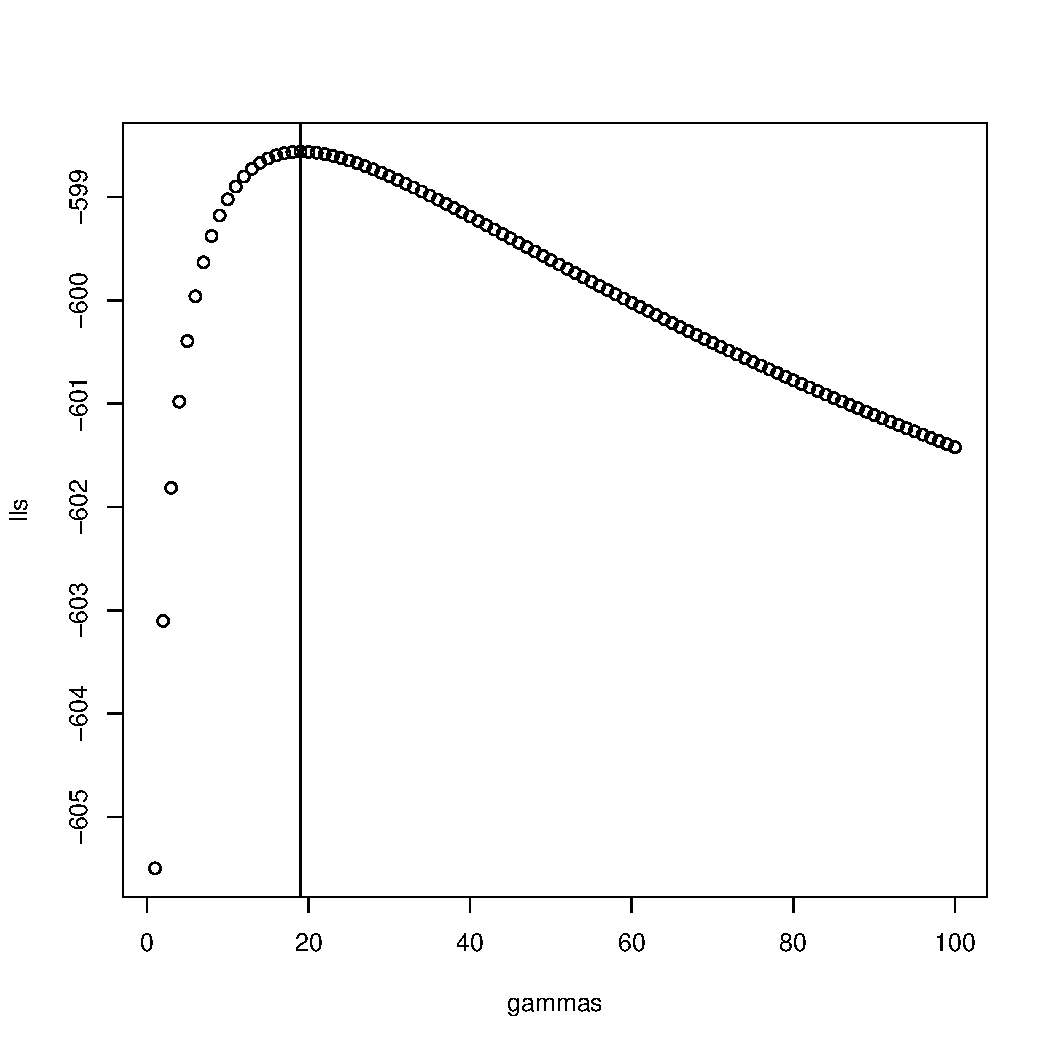
\includegraphics[width=3.7in,height=2.8in]{figure/PS11-unnamed-chunk-6-1} 

}



\end{knitrout}


\item What is the substantive interpretation of the maximum likelihood estimates of $\gamma$ and $\beta_1$? (Note that the standard errors using this method understate the true sampling variability because they are conditional on a particular choice of $\gamma$. Ignore the reported standard errors, and just interpret the estimates.)\\
Answer:\\
The maximum likelihood estimate of $\gamma$ is 19 shillings, which suggests that redeeming the voucher involves some transaction cost even when the nominal price is very small.  The coefficient on the treatment variable, $ln(price+19)$, is -1.98, which suggests that for every one unit change in this rescaled version of the treatment, the log-odds of purchase declines by -1.98.  For example, suppose that the offer price rises from 0 to 100 shillings.  The $ln(price+19)$ would change from 2.94 to 4.78, and this change would reduce the log-odds of purchase by 3.63.To illustrate what this means in terms of percentage points, suppose that a person has a 50\% chance of making a purchase at a price of zero (50\% implies a log-odds of 0). If that person were to be offered a price of 100, the predicted probability of a purchase is $1/(1+e^(-3.63) )=0.026$, or 2.6\%. 


\end{enumerate}
\section*{Question 10}
This chapter discussed the modeling issues that arise when randomly assigned treatments vary in intensity or duration. The table below considers a different case, where subjects are randomly assigned treatments but then choose to take different dosages. In this experiment, subjects were randomly assigned to receive one of two pre-recorded phone messages.\footnote{Gerber et al. 2010.} The treatment script encouraged people to vote and revealed whether members of the household voted in the past two elections. The control script encouraged people to recycle. Both calls were made the day before the election. Both calls were answered at similar rates. The table below presents voting rates for households that answered the phone call. Voting rates are broken down by how long the person answering the phone took to hang up after the recorded message began.

% Table generated by Excel2LaTeX from sheet 'Sheet1'
\begin{table}[htbp]
  \centering
  \caption{Question 10 Table}
    \begin{tabular}{rrrrrr}
    \toprule
          & \multicolumn{5}{c}{Duration of call before respondent disconnected } \\
    \midrule
    Treatment group  & 1-10 seconds  & 11-20 seconds  & 21-30 seconds  & 31-40 seconds  & Total  \\
    Call encouraged voting  & 16.6 (187)  & 17.4 (784)  & 19.7 (983)  & 24.3 (2,032)  & 21.4 (3,986)  \\
    Call encouraged recycling  & 17.5 (143)  & 18.3 (619)  & 18.9 (1,132)  & 19.8 (2,012)  & 19.2 (3,906)  \\
    \bottomrule
    \multicolumn{6}{l}{Entries are percent voting, with Ns in parentheses. The sample is restricted to one-voter households.}\\
        \multicolumn{6}{l}{Both scripts were approximately 35 seconds long.}\\
    \end{tabular}%
  \label{tab:addlabel}%
\end{table}%

\begin{enumerate}[a)]
\item Focusing only on households than answered the phone, estimate the apparent average effect of assignment to the script that encouraged voting?\\
Answer:\\
The estimated ATE is 21.4 - 19.2 = 2.2 percentage points.


\item Does this table provide convincing evidence that ``the longer a person listens to a recorded message that encourages voting, the more effective that message will be in terms of boosting voter turnout?'' Why or why not?\\
Answer:\\
No. The length of time one listens before hanging up is not randomly assigned, and the people who listen for a given length of time to one script are not necessarily comparable in terms of potential outcomes to those who listen the same length of time to the other script. For example, it may be that people who are very interested in politics (and very likely to vote) listen to the entire voting script but do not listen to the entire recycling script. We cannot infer anything about the effect of listening duration from these results unless we impose some strong assumptions that do not follow from the experimental design. 

\end{enumerate}


\end{document}

